\begin{figure}[H] \centering % Created by tikzDevice version 0.12.4 on 2023-08-13 18:11:40
% !TEX encoding = UTF-8 Unicode
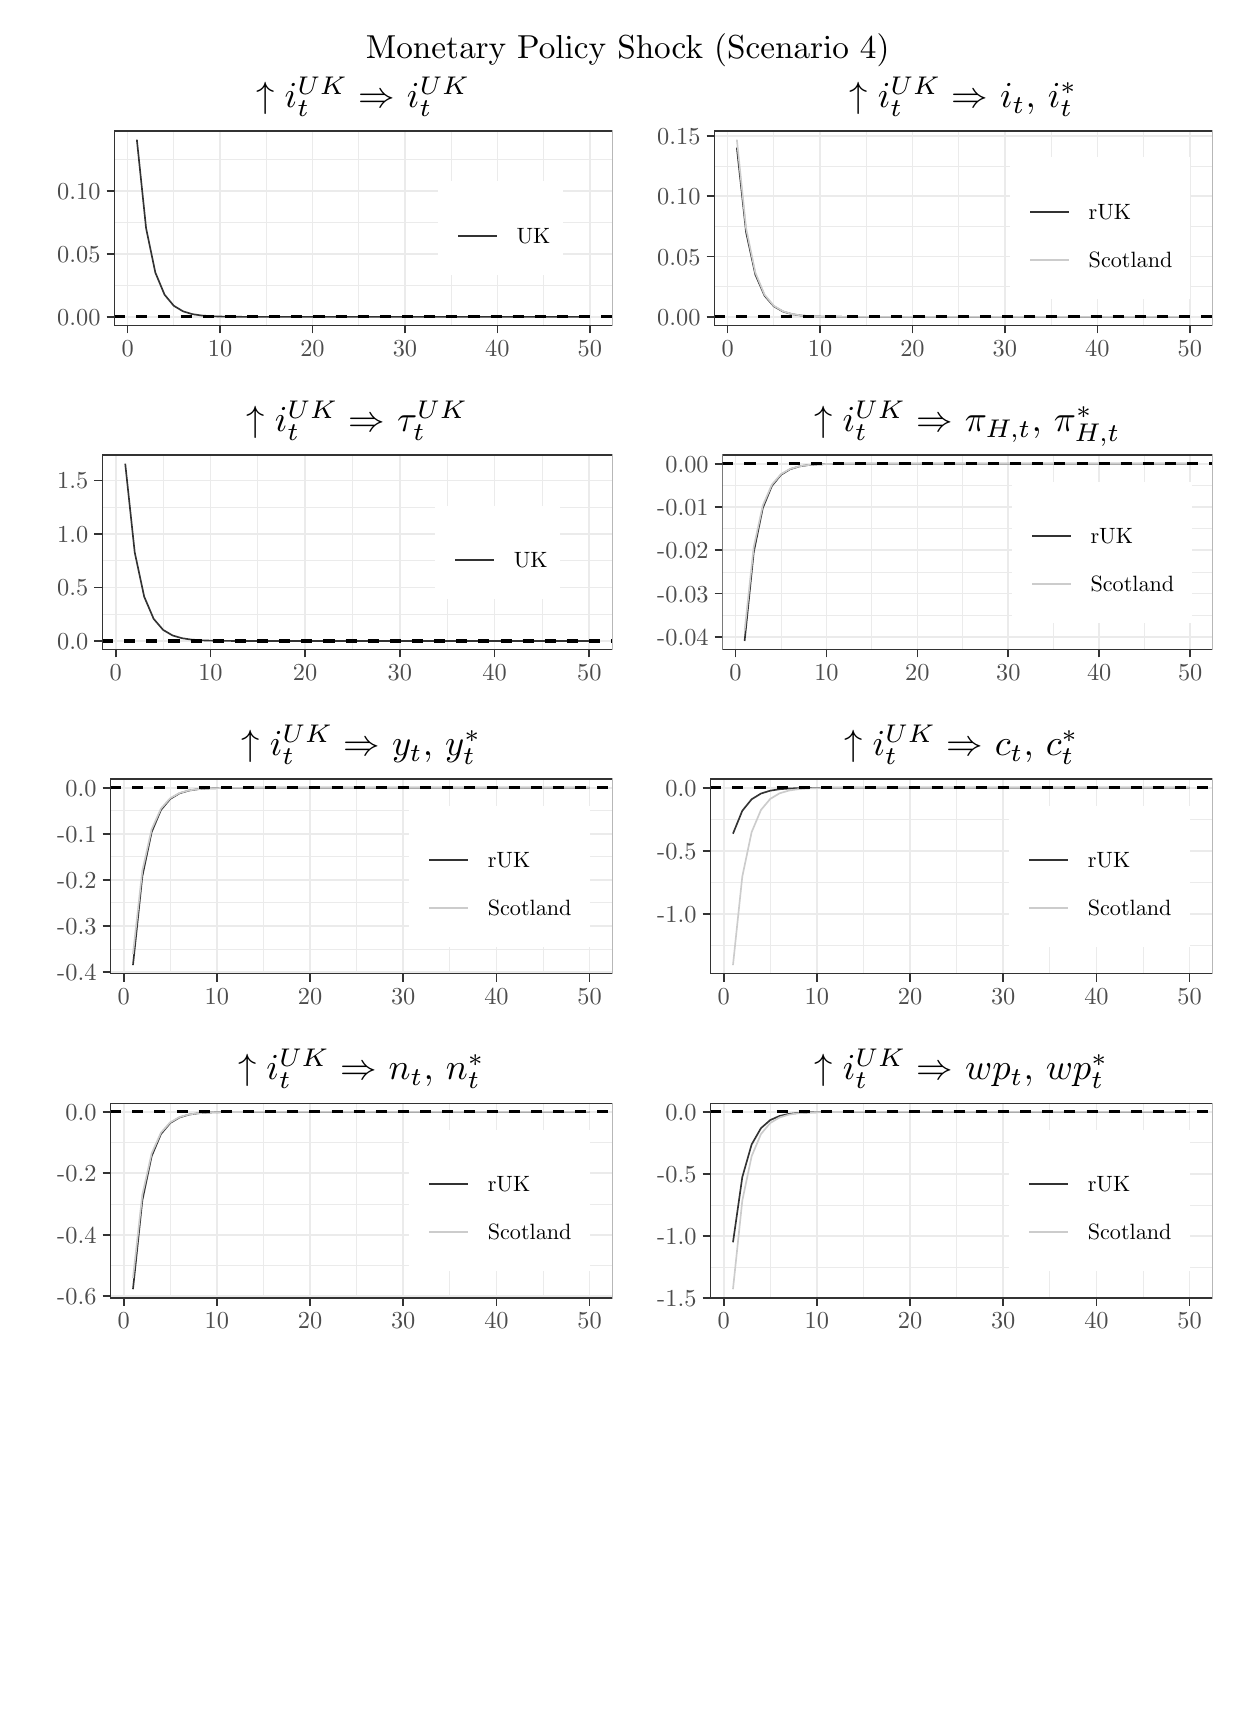
\begin{tikzpicture}[x=1pt,y=1pt]
\definecolor{fillColor}{RGB}{255,255,255}
\path[use as bounding box,fill=fillColor,fill opacity=0.00] (0,0) rectangle (433.62,599.84);
\begin{scope}
\path[clip] (  0.00,468.44) rectangle (216.81,585.55);
\definecolor{drawColor}{RGB}{255,255,255}
\definecolor{fillColor}{RGB}{255,255,255}

\path[draw=drawColor,line width= 0.6pt,line join=round,line cap=round,fill=fillColor] (  0.00,468.44) rectangle (216.81,585.55);
\end{scope}
\begin{scope}
\path[clip] ( 31.27,492.12) rectangle (211.31,562.59);
\definecolor{fillColor}{RGB}{255,255,255}

\path[fill=fillColor] ( 31.27,492.12) rectangle (211.31,562.59);
\definecolor{drawColor}{gray}{0.92}

\path[draw=drawColor,line width= 0.3pt,line join=round] ( 31.27,506.68) --
	(211.31,506.68);

\path[draw=drawColor,line width= 0.3pt,line join=round] ( 31.27,529.39) --
	(211.31,529.39);

\path[draw=drawColor,line width= 0.3pt,line join=round] ( 31.27,552.10) --
	(211.31,552.10);

\path[draw=drawColor,line width= 0.3pt,line join=round] ( 52.81,492.12) --
	( 52.81,562.59);

\path[draw=drawColor,line width= 0.3pt,line join=round] ( 86.22,492.12) --
	( 86.22,562.59);

\path[draw=drawColor,line width= 0.3pt,line join=round] (119.62,492.12) --
	(119.62,562.59);

\path[draw=drawColor,line width= 0.3pt,line join=round] (153.02,492.12) --
	(153.02,562.59);

\path[draw=drawColor,line width= 0.3pt,line join=round] (186.43,492.12) --
	(186.43,562.59);

\path[draw=drawColor,line width= 0.6pt,line join=round] ( 31.27,495.32) --
	(211.31,495.32);

\path[draw=drawColor,line width= 0.6pt,line join=round] ( 31.27,518.04) --
	(211.31,518.04);

\path[draw=drawColor,line width= 0.6pt,line join=round] ( 31.27,540.75) --
	(211.31,540.75);

\path[draw=drawColor,line width= 0.6pt,line join=round] ( 36.11,492.12) --
	( 36.11,562.59);

\path[draw=drawColor,line width= 0.6pt,line join=round] ( 69.52,492.12) --
	( 69.52,562.59);

\path[draw=drawColor,line width= 0.6pt,line join=round] (102.92,492.12) --
	(102.92,562.59);

\path[draw=drawColor,line width= 0.6pt,line join=round] (136.32,492.12) --
	(136.32,562.59);

\path[draw=drawColor,line width= 0.6pt,line join=round] (169.72,492.12) --
	(169.72,562.59);

\path[draw=drawColor,line width= 0.6pt,line join=round] (203.13,492.12) --
	(203.13,562.59);
\definecolor{drawColor}{gray}{0.20}

\path[draw=drawColor,line width= 0.6pt,line join=round] ( 39.45,559.39) --
	( 42.79,527.36) --
	( 46.13,511.34) --
	( 49.47,503.33) --
	( 52.81,499.33) --
	( 56.15,497.33) --
	( 59.50,496.32) --
	( 62.84,495.82) --
	( 66.18,495.57) --
	( 69.52,495.45) --
	( 72.86,495.39) --
	( 76.20,495.35) --
	( 79.54,495.34) --
	( 82.88,495.33) --
	( 86.22,495.33) --
	( 89.56,495.33) --
	( 92.90,495.32) --
	( 96.24,495.32) --
	( 99.58,495.32) --
	(102.92,495.32) --
	(106.26,495.32) --
	(109.60,495.32) --
	(112.94,495.32) --
	(116.28,495.32) --
	(119.62,495.32) --
	(122.96,495.32) --
	(126.30,495.32) --
	(129.64,495.32) --
	(132.98,495.32) --
	(136.32,495.32) --
	(139.66,495.32) --
	(143.00,495.32) --
	(146.34,495.32) --
	(149.68,495.32) --
	(153.02,495.32) --
	(156.36,495.32) --
	(159.70,495.32) --
	(163.04,495.32) --
	(166.38,495.32) --
	(169.72,495.32) --
	(173.06,495.32) --
	(176.40,495.32) --
	(179.74,495.32) --
	(183.08,495.32) --
	(186.43,495.32) --
	(189.77,495.32) --
	(193.11,495.32) --
	(196.45,495.32) --
	(199.79,495.32) --
	(203.13,495.32);
\definecolor{drawColor}{RGB}{0,0,0}

\path[draw=drawColor,line width= 1.1pt,dash pattern=on 4pt off 4pt ,line join=round] ( 31.27,495.32) -- (211.31,495.32);
\definecolor{drawColor}{gray}{0.20}

\path[draw=drawColor,line width= 0.6pt,line join=round,line cap=round] ( 31.27,492.12) rectangle (211.31,562.59);
\end{scope}
\begin{scope}
\path[clip] (  0.00,  0.00) rectangle (433.62,599.84);
\definecolor{drawColor}{gray}{0.30}

\node[text=drawColor,anchor=base east,inner sep=0pt, outer sep=0pt, scale=  0.88] at ( 26.32,492.29) {0.00};

\node[text=drawColor,anchor=base east,inner sep=0pt, outer sep=0pt, scale=  0.88] at ( 26.32,515.00) {0.05};

\node[text=drawColor,anchor=base east,inner sep=0pt, outer sep=0pt, scale=  0.88] at ( 26.32,537.72) {0.10};
\end{scope}
\begin{scope}
\path[clip] (  0.00,  0.00) rectangle (433.62,599.84);
\definecolor{drawColor}{gray}{0.20}

\path[draw=drawColor,line width= 0.6pt,line join=round] ( 28.52,495.32) --
	( 31.27,495.32);

\path[draw=drawColor,line width= 0.6pt,line join=round] ( 28.52,518.04) --
	( 31.27,518.04);

\path[draw=drawColor,line width= 0.6pt,line join=round] ( 28.52,540.75) --
	( 31.27,540.75);
\end{scope}
\begin{scope}
\path[clip] (  0.00,  0.00) rectangle (433.62,599.84);
\definecolor{drawColor}{gray}{0.20}

\path[draw=drawColor,line width= 0.6pt,line join=round] ( 36.11,489.37) --
	( 36.11,492.12);

\path[draw=drawColor,line width= 0.6pt,line join=round] ( 69.52,489.37) --
	( 69.52,492.12);

\path[draw=drawColor,line width= 0.6pt,line join=round] (102.92,489.37) --
	(102.92,492.12);

\path[draw=drawColor,line width= 0.6pt,line join=round] (136.32,489.37) --
	(136.32,492.12);

\path[draw=drawColor,line width= 0.6pt,line join=round] (169.72,489.37) --
	(169.72,492.12);

\path[draw=drawColor,line width= 0.6pt,line join=round] (203.13,489.37) --
	(203.13,492.12);
\end{scope}
\begin{scope}
\path[clip] (  0.00,  0.00) rectangle (433.62,599.84);
\definecolor{drawColor}{gray}{0.30}

\node[text=drawColor,anchor=base,inner sep=0pt, outer sep=0pt, scale=  0.88] at ( 36.11,481.11) {0};

\node[text=drawColor,anchor=base,inner sep=0pt, outer sep=0pt, scale=  0.88] at ( 69.52,481.11) {10};

\node[text=drawColor,anchor=base,inner sep=0pt, outer sep=0pt, scale=  0.88] at (102.92,481.11) {20};

\node[text=drawColor,anchor=base,inner sep=0pt, outer sep=0pt, scale=  0.88] at (136.32,481.11) {30};

\node[text=drawColor,anchor=base,inner sep=0pt, outer sep=0pt, scale=  0.88] at (169.72,481.11) {40};

\node[text=drawColor,anchor=base,inner sep=0pt, outer sep=0pt, scale=  0.88] at (203.13,481.11) {50};
\end{scope}
\begin{scope}
\path[clip] (  0.00,  0.00) rectangle (433.62,599.84);
\definecolor{fillColor}{RGB}{255,255,255}

\path[fill=fillColor] (148.30,510.43) rectangle (193.30,544.28);
\end{scope}
\begin{scope}
\path[clip] (  0.00,  0.00) rectangle (433.62,599.84);
\definecolor{fillColor}{RGB}{255,255,255}

\path[fill=fillColor] (153.80,515.93) rectangle (171.15,533.28);
\end{scope}
\begin{scope}
\path[clip] (  0.00,  0.00) rectangle (433.62,599.84);
\definecolor{drawColor}{gray}{0.20}

\path[draw=drawColor,line width= 0.6pt,line join=round] (155.54,524.61) -- (169.41,524.61);
\end{scope}
\begin{scope}
\path[clip] (  0.00,  0.00) rectangle (433.62,599.84);
\definecolor{drawColor}{RGB}{0,0,0}

\node[text=drawColor,anchor=base west,inner sep=0pt, outer sep=0pt, scale=  0.80] at (176.65,521.85) {UK};
\end{scope}
\begin{scope}
\path[clip] (  0.00,  0.00) rectangle (433.62,599.84);
\definecolor{drawColor}{RGB}{0,0,0}

\node[text=drawColor,anchor=base,inner sep=0pt, outer sep=0pt, scale=  1.32] at (121.29,570.96) {$\uparrow  i^{UK}_t \Rightarrow $ ${i^{UK}_t}$};
\end{scope}
\begin{scope}
\path[clip] (216.81,468.44) rectangle (433.62,585.55);
\definecolor{drawColor}{RGB}{255,255,255}
\definecolor{fillColor}{RGB}{255,255,255}

\path[draw=drawColor,line width= 0.6pt,line join=round,line cap=round,fill=fillColor] (216.81,468.44) rectangle (433.62,585.55);
\end{scope}
\begin{scope}
\path[clip] (248.08,492.12) rectangle (428.12,562.59);
\definecolor{fillColor}{RGB}{255,255,255}

\path[fill=fillColor] (248.08,492.12) rectangle (428.12,562.59);
\definecolor{drawColor}{gray}{0.92}

\path[draw=drawColor,line width= 0.3pt,line join=round] (248.08,506.22) --
	(428.12,506.22);

\path[draw=drawColor,line width= 0.3pt,line join=round] (248.08,528.00) --
	(428.12,528.00);

\path[draw=drawColor,line width= 0.3pt,line join=round] (248.08,549.78) --
	(428.12,549.78);

\path[draw=drawColor,line width= 0.3pt,line join=round] (269.62,492.12) --
	(269.62,562.59);

\path[draw=drawColor,line width= 0.3pt,line join=round] (303.03,492.12) --
	(303.03,562.59);

\path[draw=drawColor,line width= 0.3pt,line join=round] (336.43,492.12) --
	(336.43,562.59);

\path[draw=drawColor,line width= 0.3pt,line join=round] (369.83,492.12) --
	(369.83,562.59);

\path[draw=drawColor,line width= 0.3pt,line join=round] (403.24,492.12) --
	(403.24,562.59);

\path[draw=drawColor,line width= 0.6pt,line join=round] (248.08,495.32) --
	(428.12,495.32);

\path[draw=drawColor,line width= 0.6pt,line join=round] (248.08,517.11) --
	(428.12,517.11);

\path[draw=drawColor,line width= 0.6pt,line join=round] (248.08,538.89) --
	(428.12,538.89);

\path[draw=drawColor,line width= 0.6pt,line join=round] (248.08,560.67) --
	(428.12,560.67);

\path[draw=drawColor,line width= 0.6pt,line join=round] (252.92,492.12) --
	(252.92,562.59);

\path[draw=drawColor,line width= 0.6pt,line join=round] (286.33,492.12) --
	(286.33,562.59);

\path[draw=drawColor,line width= 0.6pt,line join=round] (319.73,492.12) --
	(319.73,562.59);

\path[draw=drawColor,line width= 0.6pt,line join=round] (353.13,492.12) --
	(353.13,562.59);

\path[draw=drawColor,line width= 0.6pt,line join=round] (386.53,492.12) --
	(386.53,562.59);

\path[draw=drawColor,line width= 0.6pt,line join=round] (419.94,492.12) --
	(419.94,562.59);
\definecolor{drawColor}{gray}{0.20}

\path[draw=drawColor,line width= 0.6pt,line join=round] (256.26,556.52) --
	(259.60,525.92) --
	(262.94,510.62) --
	(266.28,502.97) --
	(269.62,499.15) --
	(272.96,497.24) --
	(276.31,496.28) --
	(279.65,495.80) --
	(282.99,495.56) --
	(286.33,495.44) --
	(289.67,495.38) --
	(293.01,495.35) --
	(296.35,495.34) --
	(299.69,495.33) --
	(303.03,495.33) --
	(306.37,495.33) --
	(309.71,495.32) --
	(313.05,495.32) --
	(316.39,495.32) --
	(319.73,495.32) --
	(323.07,495.32) --
	(326.41,495.32) --
	(329.75,495.32) --
	(333.09,495.32) --
	(336.43,495.32) --
	(339.77,495.32) --
	(343.11,495.32) --
	(346.45,495.32) --
	(349.79,495.32) --
	(353.13,495.32) --
	(356.47,495.32) --
	(359.81,495.32) --
	(363.15,495.32) --
	(366.49,495.32) --
	(369.83,495.32) --
	(373.17,495.32) --
	(376.51,495.32) --
	(379.85,495.32) --
	(383.19,495.32) --
	(386.53,495.32) --
	(389.87,495.32) --
	(393.21,495.32) --
	(396.55,495.32) --
	(399.89,495.32) --
	(403.24,495.32) --
	(406.58,495.32) --
	(409.92,495.32) --
	(413.26,495.32) --
	(416.60,495.32) --
	(419.94,495.32);
\definecolor{drawColor}{gray}{0.80}

\path[draw=drawColor,line width= 0.6pt,line join=round] (256.26,559.39) --
	(259.60,527.36) --
	(262.94,511.34) --
	(266.28,503.33) --
	(269.62,499.33) --
	(272.96,497.33) --
	(276.31,496.32) --
	(279.65,495.82) --
	(282.99,495.57) --
	(286.33,495.45) --
	(289.67,495.39) --
	(293.01,495.35) --
	(296.35,495.34) --
	(299.69,495.33) --
	(303.03,495.33) --
	(306.37,495.33) --
	(309.71,495.32) --
	(313.05,495.32) --
	(316.39,495.32) --
	(319.73,495.32) --
	(323.07,495.32) --
	(326.41,495.32) --
	(329.75,495.32) --
	(333.09,495.32) --
	(336.43,495.32) --
	(339.77,495.32) --
	(343.11,495.32) --
	(346.45,495.32) --
	(349.79,495.32) --
	(353.13,495.32) --
	(356.47,495.32) --
	(359.81,495.32) --
	(363.15,495.32) --
	(366.49,495.32) --
	(369.83,495.32) --
	(373.17,495.32) --
	(376.51,495.32) --
	(379.85,495.32) --
	(383.19,495.32) --
	(386.53,495.32) --
	(389.87,495.32) --
	(393.21,495.32) --
	(396.55,495.32) --
	(399.89,495.32) --
	(403.24,495.32) --
	(406.58,495.32) --
	(409.92,495.32) --
	(413.26,495.32) --
	(416.60,495.32) --
	(419.94,495.32);
\definecolor{drawColor}{RGB}{0,0,0}

\path[draw=drawColor,line width= 1.1pt,dash pattern=on 4pt off 4pt ,line join=round] (248.08,495.32) -- (428.12,495.32);
\definecolor{drawColor}{gray}{0.20}

\path[draw=drawColor,line width= 0.6pt,line join=round,line cap=round] (248.08,492.12) rectangle (428.12,562.59);
\end{scope}
\begin{scope}
\path[clip] (  0.00,  0.00) rectangle (433.62,599.84);
\definecolor{drawColor}{gray}{0.30}

\node[text=drawColor,anchor=base east,inner sep=0pt, outer sep=0pt, scale=  0.88] at (243.13,492.29) {0.00};

\node[text=drawColor,anchor=base east,inner sep=0pt, outer sep=0pt, scale=  0.88] at (243.13,514.08) {0.05};

\node[text=drawColor,anchor=base east,inner sep=0pt, outer sep=0pt, scale=  0.88] at (243.13,535.86) {0.10};

\node[text=drawColor,anchor=base east,inner sep=0pt, outer sep=0pt, scale=  0.88] at (243.13,557.64) {0.15};
\end{scope}
\begin{scope}
\path[clip] (  0.00,  0.00) rectangle (433.62,599.84);
\definecolor{drawColor}{gray}{0.20}

\path[draw=drawColor,line width= 0.6pt,line join=round] (245.33,495.32) --
	(248.08,495.32);

\path[draw=drawColor,line width= 0.6pt,line join=round] (245.33,517.11) --
	(248.08,517.11);

\path[draw=drawColor,line width= 0.6pt,line join=round] (245.33,538.89) --
	(248.08,538.89);

\path[draw=drawColor,line width= 0.6pt,line join=round] (245.33,560.67) --
	(248.08,560.67);
\end{scope}
\begin{scope}
\path[clip] (  0.00,  0.00) rectangle (433.62,599.84);
\definecolor{drawColor}{gray}{0.20}

\path[draw=drawColor,line width= 0.6pt,line join=round] (252.92,489.37) --
	(252.92,492.12);

\path[draw=drawColor,line width= 0.6pt,line join=round] (286.33,489.37) --
	(286.33,492.12);

\path[draw=drawColor,line width= 0.6pt,line join=round] (319.73,489.37) --
	(319.73,492.12);

\path[draw=drawColor,line width= 0.6pt,line join=round] (353.13,489.37) --
	(353.13,492.12);

\path[draw=drawColor,line width= 0.6pt,line join=round] (386.53,489.37) --
	(386.53,492.12);

\path[draw=drawColor,line width= 0.6pt,line join=round] (419.94,489.37) --
	(419.94,492.12);
\end{scope}
\begin{scope}
\path[clip] (  0.00,  0.00) rectangle (433.62,599.84);
\definecolor{drawColor}{gray}{0.30}

\node[text=drawColor,anchor=base,inner sep=0pt, outer sep=0pt, scale=  0.88] at (252.92,481.11) {0};

\node[text=drawColor,anchor=base,inner sep=0pt, outer sep=0pt, scale=  0.88] at (286.33,481.11) {10};

\node[text=drawColor,anchor=base,inner sep=0pt, outer sep=0pt, scale=  0.88] at (319.73,481.11) {20};

\node[text=drawColor,anchor=base,inner sep=0pt, outer sep=0pt, scale=  0.88] at (353.13,481.11) {30};

\node[text=drawColor,anchor=base,inner sep=0pt, outer sep=0pt, scale=  0.88] at (386.53,481.11) {40};

\node[text=drawColor,anchor=base,inner sep=0pt, outer sep=0pt, scale=  0.88] at (419.94,481.11) {50};
\end{scope}
\begin{scope}
\path[clip] (  0.00,  0.00) rectangle (433.62,599.84);
\definecolor{fillColor}{RGB}{255,255,255}

\path[fill=fillColor] (355.07,501.76) rectangle (420.16,552.95);
\end{scope}
\begin{scope}
\path[clip] (  0.00,  0.00) rectangle (433.62,599.84);
\definecolor{fillColor}{RGB}{255,255,255}

\path[fill=fillColor] (360.57,524.61) rectangle (377.91,541.95);
\end{scope}
\begin{scope}
\path[clip] (  0.00,  0.00) rectangle (433.62,599.84);
\definecolor{drawColor}{gray}{0.20}

\path[draw=drawColor,line width= 0.6pt,line join=round] (362.30,533.28) -- (376.18,533.28);
\end{scope}
\begin{scope}
\path[clip] (  0.00,  0.00) rectangle (433.62,599.84);
\definecolor{fillColor}{RGB}{255,255,255}

\path[fill=fillColor] (360.57,507.26) rectangle (377.91,524.61);
\end{scope}
\begin{scope}
\path[clip] (  0.00,  0.00) rectangle (433.62,599.84);
\definecolor{drawColor}{gray}{0.80}

\path[draw=drawColor,line width= 0.6pt,line join=round] (362.30,515.93) -- (376.18,515.93);
\end{scope}
\begin{scope}
\path[clip] (  0.00,  0.00) rectangle (433.62,599.84);
\definecolor{drawColor}{RGB}{0,0,0}

\node[text=drawColor,anchor=base west,inner sep=0pt, outer sep=0pt, scale=  0.80] at (383.41,530.52) {rUK};
\end{scope}
\begin{scope}
\path[clip] (  0.00,  0.00) rectangle (433.62,599.84);
\definecolor{drawColor}{RGB}{0,0,0}

\node[text=drawColor,anchor=base west,inner sep=0pt, outer sep=0pt, scale=  0.80] at (383.41,513.18) {Scotland};
\end{scope}
\begin{scope}
\path[clip] (  0.00,  0.00) rectangle (433.62,599.84);
\definecolor{drawColor}{RGB}{0,0,0}

\node[text=drawColor,anchor=base,inner sep=0pt, outer sep=0pt, scale=  1.32] at (338.10,570.96) {$\uparrow  i^{UK}_t \Rightarrow $ ${i_t}$, ${i^*_t}$};
\end{scope}
\begin{scope}
\path[clip] (  0.00,351.33) rectangle (216.81,468.44);
\definecolor{drawColor}{RGB}{255,255,255}
\definecolor{fillColor}{RGB}{255,255,255}

\path[draw=drawColor,line width= 0.6pt,line join=round,line cap=round,fill=fillColor] (  0.00,351.33) rectangle (216.81,468.44);
\end{scope}
\begin{scope}
\path[clip] ( 26.87,375.01) rectangle (211.31,445.48);
\definecolor{fillColor}{RGB}{255,255,255}

\path[fill=fillColor] ( 26.87,375.01) rectangle (211.31,445.48);
\definecolor{drawColor}{gray}{0.92}

\path[draw=drawColor,line width= 0.3pt,line join=round] ( 26.87,387.87) --
	(211.31,387.87);

\path[draw=drawColor,line width= 0.3pt,line join=round] ( 26.87,407.19) --
	(211.31,407.19);

\path[draw=drawColor,line width= 0.3pt,line join=round] ( 26.87,426.51) --
	(211.31,426.51);

\path[draw=drawColor,line width= 0.3pt,line join=round] ( 48.94,375.01) --
	( 48.94,445.48);

\path[draw=drawColor,line width= 0.3pt,line join=round] ( 83.16,375.01) --
	( 83.16,445.48);

\path[draw=drawColor,line width= 0.3pt,line join=round] (117.38,375.01) --
	(117.38,445.48);

\path[draw=drawColor,line width= 0.3pt,line join=round] (151.60,375.01) --
	(151.60,445.48);

\path[draw=drawColor,line width= 0.3pt,line join=round] (185.82,375.01) --
	(185.82,445.48);

\path[draw=drawColor,line width= 0.6pt,line join=round] ( 26.87,378.21) --
	(211.31,378.21);

\path[draw=drawColor,line width= 0.6pt,line join=round] ( 26.87,397.53) --
	(211.31,397.53);

\path[draw=drawColor,line width= 0.6pt,line join=round] ( 26.87,416.85) --
	(211.31,416.85);

\path[draw=drawColor,line width= 0.6pt,line join=round] ( 26.87,436.17) --
	(211.31,436.17);

\path[draw=drawColor,line width= 0.6pt,line join=round] ( 31.83,375.01) --
	( 31.83,445.48);

\path[draw=drawColor,line width= 0.6pt,line join=round] ( 66.05,375.01) --
	( 66.05,445.48);

\path[draw=drawColor,line width= 0.6pt,line join=round] (100.27,375.01) --
	(100.27,445.48);

\path[draw=drawColor,line width= 0.6pt,line join=round] (134.49,375.01) --
	(134.49,445.48);

\path[draw=drawColor,line width= 0.6pt,line join=round] (168.71,375.01) --
	(168.71,445.48);

\path[draw=drawColor,line width= 0.6pt,line join=round] (202.93,375.01) --
	(202.93,445.48);
\definecolor{drawColor}{gray}{0.20}

\path[draw=drawColor,line width= 0.6pt,line join=round] ( 35.25,442.28) --
	( 38.68,410.25) --
	( 42.10,394.23) --
	( 45.52,386.22) --
	( 48.94,382.22) --
	( 52.36,380.21) --
	( 55.79,379.21) --
	( 59.21,378.71) --
	( 62.63,378.46) --
	( 66.05,378.34) --
	( 69.47,378.28) --
	( 72.90,378.24) --
	( 76.32,378.23) --
	( 79.74,378.22) --
	( 83.16,378.22) --
	( 86.58,378.21) --
	( 90.00,378.21) --
	( 93.43,378.21) --
	( 96.85,378.21) --
	(100.27,378.21) --
	(103.69,378.21) --
	(107.11,378.21) --
	(110.54,378.21) --
	(113.96,378.21) --
	(117.38,378.21) --
	(120.80,378.21) --
	(124.22,378.21) --
	(127.65,378.21) --
	(131.07,378.21) --
	(134.49,378.21) --
	(137.91,378.21) --
	(141.33,378.21) --
	(144.75,378.21) --
	(148.18,378.21) --
	(151.60,378.21) --
	(155.02,378.21) --
	(158.44,378.21) --
	(161.86,378.21) --
	(165.29,378.21) --
	(168.71,378.21) --
	(172.13,378.21) --
	(175.55,378.21) --
	(178.97,378.21) --
	(182.40,378.21) --
	(185.82,378.21) --
	(189.24,378.21) --
	(192.66,378.21) --
	(196.08,378.21) --
	(199.50,378.21) --
	(202.93,378.21);
\definecolor{drawColor}{RGB}{0,0,0}

\path[draw=drawColor,line width= 1.1pt,dash pattern=on 4pt off 4pt ,line join=round] ( 26.87,378.21) -- (211.31,378.21);
\definecolor{drawColor}{gray}{0.20}

\path[draw=drawColor,line width= 0.6pt,line join=round,line cap=round] ( 26.87,375.01) rectangle (211.31,445.48);
\end{scope}
\begin{scope}
\path[clip] (  0.00,  0.00) rectangle (433.62,599.84);
\definecolor{drawColor}{gray}{0.30}

\node[text=drawColor,anchor=base east,inner sep=0pt, outer sep=0pt, scale=  0.88] at ( 21.92,375.18) {0.0};

\node[text=drawColor,anchor=base east,inner sep=0pt, outer sep=0pt, scale=  0.88] at ( 21.92,394.50) {0.5};

\node[text=drawColor,anchor=base east,inner sep=0pt, outer sep=0pt, scale=  0.88] at ( 21.92,413.82) {1.0};

\node[text=drawColor,anchor=base east,inner sep=0pt, outer sep=0pt, scale=  0.88] at ( 21.92,433.14) {1.5};
\end{scope}
\begin{scope}
\path[clip] (  0.00,  0.00) rectangle (433.62,599.84);
\definecolor{drawColor}{gray}{0.20}

\path[draw=drawColor,line width= 0.6pt,line join=round] ( 24.12,378.21) --
	( 26.87,378.21);

\path[draw=drawColor,line width= 0.6pt,line join=round] ( 24.12,397.53) --
	( 26.87,397.53);

\path[draw=drawColor,line width= 0.6pt,line join=round] ( 24.12,416.85) --
	( 26.87,416.85);

\path[draw=drawColor,line width= 0.6pt,line join=round] ( 24.12,436.17) --
	( 26.87,436.17);
\end{scope}
\begin{scope}
\path[clip] (  0.00,  0.00) rectangle (433.62,599.84);
\definecolor{drawColor}{gray}{0.20}

\path[draw=drawColor,line width= 0.6pt,line join=round] ( 31.83,372.26) --
	( 31.83,375.01);

\path[draw=drawColor,line width= 0.6pt,line join=round] ( 66.05,372.26) --
	( 66.05,375.01);

\path[draw=drawColor,line width= 0.6pt,line join=round] (100.27,372.26) --
	(100.27,375.01);

\path[draw=drawColor,line width= 0.6pt,line join=round] (134.49,372.26) --
	(134.49,375.01);

\path[draw=drawColor,line width= 0.6pt,line join=round] (168.71,372.26) --
	(168.71,375.01);

\path[draw=drawColor,line width= 0.6pt,line join=round] (202.93,372.26) --
	(202.93,375.01);
\end{scope}
\begin{scope}
\path[clip] (  0.00,  0.00) rectangle (433.62,599.84);
\definecolor{drawColor}{gray}{0.30}

\node[text=drawColor,anchor=base,inner sep=0pt, outer sep=0pt, scale=  0.88] at ( 31.83,364.00) {0};

\node[text=drawColor,anchor=base,inner sep=0pt, outer sep=0pt, scale=  0.88] at ( 66.05,364.00) {10};

\node[text=drawColor,anchor=base,inner sep=0pt, outer sep=0pt, scale=  0.88] at (100.27,364.00) {20};

\node[text=drawColor,anchor=base,inner sep=0pt, outer sep=0pt, scale=  0.88] at (134.49,364.00) {30};

\node[text=drawColor,anchor=base,inner sep=0pt, outer sep=0pt, scale=  0.88] at (168.71,364.00) {40};

\node[text=drawColor,anchor=base,inner sep=0pt, outer sep=0pt, scale=  0.88] at (202.93,364.00) {50};
\end{scope}
\begin{scope}
\path[clip] (  0.00,  0.00) rectangle (433.62,599.84);
\definecolor{fillColor}{RGB}{255,255,255}

\path[fill=fillColor] (147.31,393.32) rectangle (192.31,427.17);
\end{scope}
\begin{scope}
\path[clip] (  0.00,  0.00) rectangle (433.62,599.84);
\definecolor{fillColor}{RGB}{255,255,255}

\path[fill=fillColor] (152.81,398.82) rectangle (170.16,416.17);
\end{scope}
\begin{scope}
\path[clip] (  0.00,  0.00) rectangle (433.62,599.84);
\definecolor{drawColor}{gray}{0.20}

\path[draw=drawColor,line width= 0.6pt,line join=round] (154.55,407.50) -- (168.42,407.50);
\end{scope}
\begin{scope}
\path[clip] (  0.00,  0.00) rectangle (433.62,599.84);
\definecolor{drawColor}{RGB}{0,0,0}

\node[text=drawColor,anchor=base west,inner sep=0pt, outer sep=0pt, scale=  0.80] at (175.66,404.74) {UK};
\end{scope}
\begin{scope}
\path[clip] (  0.00,  0.00) rectangle (433.62,599.84);
\definecolor{drawColor}{RGB}{0,0,0}

\node[text=drawColor,anchor=base,inner sep=0pt, outer sep=0pt, scale=  1.32] at (119.09,453.85) {$\uparrow  i^{UK}_t \Rightarrow $ ${\tau^{UK}_t}$};
\end{scope}
\begin{scope}
\path[clip] (216.81,351.33) rectangle (433.62,468.44);
\definecolor{drawColor}{RGB}{255,255,255}
\definecolor{fillColor}{RGB}{255,255,255}

\path[draw=drawColor,line width= 0.6pt,line join=round,line cap=round,fill=fillColor] (216.81,351.33) rectangle (433.62,468.44);
\end{scope}
\begin{scope}
\path[clip] (251.01,375.01) rectangle (428.12,445.48);
\definecolor{fillColor}{RGB}{255,255,255}

\path[fill=fillColor] (251.01,375.01) rectangle (428.12,445.48);
\definecolor{drawColor}{gray}{0.92}

\path[draw=drawColor,line width= 0.3pt,line join=round] (251.01,387.50) --
	(428.12,387.50);

\path[draw=drawColor,line width= 0.3pt,line join=round] (251.01,403.15) --
	(428.12,403.15);

\path[draw=drawColor,line width= 0.3pt,line join=round] (251.01,418.80) --
	(428.12,418.80);

\path[draw=drawColor,line width= 0.3pt,line join=round] (251.01,434.45) --
	(428.12,434.45);

\path[draw=drawColor,line width= 0.3pt,line join=round] (272.21,375.01) --
	(272.21,445.48);

\path[draw=drawColor,line width= 0.3pt,line join=round] (305.06,375.01) --
	(305.06,445.48);

\path[draw=drawColor,line width= 0.3pt,line join=round] (337.92,375.01) --
	(337.92,445.48);

\path[draw=drawColor,line width= 0.3pt,line join=round] (370.78,375.01) --
	(370.78,445.48);

\path[draw=drawColor,line width= 0.3pt,line join=round] (403.64,375.01) --
	(403.64,445.48);

\path[draw=drawColor,line width= 0.6pt,line join=round] (251.01,379.68) --
	(428.12,379.68);

\path[draw=drawColor,line width= 0.6pt,line join=round] (251.01,395.33) --
	(428.12,395.33);

\path[draw=drawColor,line width= 0.6pt,line join=round] (251.01,410.98) --
	(428.12,410.98);

\path[draw=drawColor,line width= 0.6pt,line join=round] (251.01,426.63) --
	(428.12,426.63);

\path[draw=drawColor,line width= 0.6pt,line join=round] (251.01,442.28) --
	(428.12,442.28);

\path[draw=drawColor,line width= 0.6pt,line join=round] (255.78,375.01) --
	(255.78,445.48);

\path[draw=drawColor,line width= 0.6pt,line join=round] (288.64,375.01) --
	(288.64,445.48);

\path[draw=drawColor,line width= 0.6pt,line join=round] (321.49,375.01) --
	(321.49,445.48);

\path[draw=drawColor,line width= 0.6pt,line join=round] (354.35,375.01) --
	(354.35,445.48);

\path[draw=drawColor,line width= 0.6pt,line join=round] (387.21,375.01) --
	(387.21,445.48);

\path[draw=drawColor,line width= 0.6pt,line join=round] (420.07,375.01) --
	(420.07,445.48);
\definecolor{drawColor}{gray}{0.20}

\path[draw=drawColor,line width= 0.6pt,line join=round] (259.06,378.21) --
	(262.35,410.25) --
	(265.63,426.26) --
	(268.92,434.27) --
	(272.21,438.27) --
	(275.49,440.28) --
	(278.78,441.28) --
	(282.06,441.78) --
	(285.35,442.03) --
	(288.64,442.15) --
	(291.92,442.22) --
	(295.21,442.25) --
	(298.49,442.26) --
	(301.78,442.27) --
	(305.06,442.27) --
	(308.35,442.28) --
	(311.64,442.28) --
	(314.92,442.28) --
	(318.21,442.28) --
	(321.49,442.28) --
	(324.78,442.28) --
	(328.07,442.28) --
	(331.35,442.28) --
	(334.64,442.28) --
	(337.92,442.28) --
	(341.21,442.28) --
	(344.49,442.28) --
	(347.78,442.28) --
	(351.07,442.28) --
	(354.35,442.28) --
	(357.64,442.28) --
	(360.92,442.28) --
	(364.21,442.28) --
	(367.50,442.28) --
	(370.78,442.28) --
	(374.07,442.28) --
	(377.35,442.28) --
	(380.64,442.28) --
	(383.93,442.28) --
	(387.21,442.28) --
	(390.50,442.28) --
	(393.78,442.28) --
	(397.07,442.28) --
	(400.35,442.28) --
	(403.64,442.28) --
	(406.93,442.28) --
	(410.21,442.28) --
	(413.50,442.28) --
	(416.78,442.28) --
	(420.07,442.28);
\definecolor{drawColor}{gray}{0.80}

\path[draw=drawColor,line width= 0.6pt,line join=round] (259.06,381.92) --
	(262.35,412.10) --
	(265.63,427.19) --
	(268.92,434.73) --
	(272.21,438.51) --
	(275.49,440.39) --
	(278.78,441.33) --
	(282.06,441.81) --
	(285.35,442.04) --
	(288.64,442.16) --
	(291.92,442.22) --
	(295.21,442.25) --
	(298.49,442.26) --
	(301.78,442.27) --
	(305.06,442.27) --
	(308.35,442.28) --
	(311.64,442.28) --
	(314.92,442.28) --
	(318.21,442.28) --
	(321.49,442.28) --
	(324.78,442.28) --
	(328.07,442.28) --
	(331.35,442.28) --
	(334.64,442.28) --
	(337.92,442.28) --
	(341.21,442.28) --
	(344.49,442.28) --
	(347.78,442.28) --
	(351.07,442.28) --
	(354.35,442.28) --
	(357.64,442.28) --
	(360.92,442.28) --
	(364.21,442.28) --
	(367.50,442.28) --
	(370.78,442.28) --
	(374.07,442.28) --
	(377.35,442.28) --
	(380.64,442.28) --
	(383.93,442.28) --
	(387.21,442.28) --
	(390.50,442.28) --
	(393.78,442.28) --
	(397.07,442.28) --
	(400.35,442.28) --
	(403.64,442.28) --
	(406.93,442.28) --
	(410.21,442.28) --
	(413.50,442.28) --
	(416.78,442.28) --
	(420.07,442.28);
\definecolor{drawColor}{RGB}{0,0,0}

\path[draw=drawColor,line width= 1.1pt,dash pattern=on 4pt off 4pt ,line join=round] (251.01,442.28) -- (428.12,442.28);
\definecolor{drawColor}{gray}{0.20}

\path[draw=drawColor,line width= 0.6pt,line join=round,line cap=round] (251.01,375.01) rectangle (428.12,445.48);
\end{scope}
\begin{scope}
\path[clip] (  0.00,  0.00) rectangle (433.62,599.84);
\definecolor{drawColor}{gray}{0.30}

\node[text=drawColor,anchor=base east,inner sep=0pt, outer sep=0pt, scale=  0.88] at (246.06,376.65) {-0.04};

\node[text=drawColor,anchor=base east,inner sep=0pt, outer sep=0pt, scale=  0.88] at (246.06,392.30) {-0.03};

\node[text=drawColor,anchor=base east,inner sep=0pt, outer sep=0pt, scale=  0.88] at (246.06,407.95) {-0.02};

\node[text=drawColor,anchor=base east,inner sep=0pt, outer sep=0pt, scale=  0.88] at (246.06,423.60) {-0.01};

\node[text=drawColor,anchor=base east,inner sep=0pt, outer sep=0pt, scale=  0.88] at (246.06,439.25) {0.00};
\end{scope}
\begin{scope}
\path[clip] (  0.00,  0.00) rectangle (433.62,599.84);
\definecolor{drawColor}{gray}{0.20}

\path[draw=drawColor,line width= 0.6pt,line join=round] (248.26,379.68) --
	(251.01,379.68);

\path[draw=drawColor,line width= 0.6pt,line join=round] (248.26,395.33) --
	(251.01,395.33);

\path[draw=drawColor,line width= 0.6pt,line join=round] (248.26,410.98) --
	(251.01,410.98);

\path[draw=drawColor,line width= 0.6pt,line join=round] (248.26,426.63) --
	(251.01,426.63);

\path[draw=drawColor,line width= 0.6pt,line join=round] (248.26,442.28) --
	(251.01,442.28);
\end{scope}
\begin{scope}
\path[clip] (  0.00,  0.00) rectangle (433.62,599.84);
\definecolor{drawColor}{gray}{0.20}

\path[draw=drawColor,line width= 0.6pt,line join=round] (255.78,372.26) --
	(255.78,375.01);

\path[draw=drawColor,line width= 0.6pt,line join=round] (288.64,372.26) --
	(288.64,375.01);

\path[draw=drawColor,line width= 0.6pt,line join=round] (321.49,372.26) --
	(321.49,375.01);

\path[draw=drawColor,line width= 0.6pt,line join=round] (354.35,372.26) --
	(354.35,375.01);

\path[draw=drawColor,line width= 0.6pt,line join=round] (387.21,372.26) --
	(387.21,375.01);

\path[draw=drawColor,line width= 0.6pt,line join=round] (420.07,372.26) --
	(420.07,375.01);
\end{scope}
\begin{scope}
\path[clip] (  0.00,  0.00) rectangle (433.62,599.84);
\definecolor{drawColor}{gray}{0.30}

\node[text=drawColor,anchor=base,inner sep=0pt, outer sep=0pt, scale=  0.88] at (255.78,364.00) {0};

\node[text=drawColor,anchor=base,inner sep=0pt, outer sep=0pt, scale=  0.88] at (288.64,364.00) {10};

\node[text=drawColor,anchor=base,inner sep=0pt, outer sep=0pt, scale=  0.88] at (321.49,364.00) {20};

\node[text=drawColor,anchor=base,inner sep=0pt, outer sep=0pt, scale=  0.88] at (354.35,364.00) {30};

\node[text=drawColor,anchor=base,inner sep=0pt, outer sep=0pt, scale=  0.88] at (387.21,364.00) {40};

\node[text=drawColor,anchor=base,inner sep=0pt, outer sep=0pt, scale=  0.88] at (420.07,364.00) {50};
\end{scope}
\begin{scope}
\path[clip] (  0.00,  0.00) rectangle (433.62,599.84);
\definecolor{fillColor}{RGB}{255,255,255}

\path[fill=fillColor] (355.73,384.65) rectangle (420.82,435.84);
\end{scope}
\begin{scope}
\path[clip] (  0.00,  0.00) rectangle (433.62,599.84);
\definecolor{fillColor}{RGB}{255,255,255}

\path[fill=fillColor] (361.23,407.50) rectangle (378.57,424.84);
\end{scope}
\begin{scope}
\path[clip] (  0.00,  0.00) rectangle (433.62,599.84);
\definecolor{drawColor}{gray}{0.20}

\path[draw=drawColor,line width= 0.6pt,line join=round] (362.96,416.17) -- (376.84,416.17);
\end{scope}
\begin{scope}
\path[clip] (  0.00,  0.00) rectangle (433.62,599.84);
\definecolor{fillColor}{RGB}{255,255,255}

\path[fill=fillColor] (361.23,390.15) rectangle (378.57,407.50);
\end{scope}
\begin{scope}
\path[clip] (  0.00,  0.00) rectangle (433.62,599.84);
\definecolor{drawColor}{gray}{0.80}

\path[draw=drawColor,line width= 0.6pt,line join=round] (362.96,398.82) -- (376.84,398.82);
\end{scope}
\begin{scope}
\path[clip] (  0.00,  0.00) rectangle (433.62,599.84);
\definecolor{drawColor}{RGB}{0,0,0}

\node[text=drawColor,anchor=base west,inner sep=0pt, outer sep=0pt, scale=  0.80] at (384.07,413.41) {rUK};
\end{scope}
\begin{scope}
\path[clip] (  0.00,  0.00) rectangle (433.62,599.84);
\definecolor{drawColor}{RGB}{0,0,0}

\node[text=drawColor,anchor=base west,inner sep=0pt, outer sep=0pt, scale=  0.80] at (384.07,396.07) {Scotland};
\end{scope}
\begin{scope}
\path[clip] (  0.00,  0.00) rectangle (433.62,599.84);
\definecolor{drawColor}{RGB}{0,0,0}

\node[text=drawColor,anchor=base,inner sep=0pt, outer sep=0pt, scale=  1.32] at (339.57,453.85) {$\uparrow  i^{UK}_t \Rightarrow $ ${\pi_{H,t}}$, ${\pi^*_{H,t}}$};
\end{scope}
\begin{scope}
\path[clip] (  0.00,234.22) rectangle (216.81,351.33);
\definecolor{drawColor}{RGB}{255,255,255}
\definecolor{fillColor}{RGB}{255,255,255}

\path[draw=drawColor,line width= 0.6pt,line join=round,line cap=round,fill=fillColor] (  0.00,234.22) rectangle (216.81,351.33);
\end{scope}
\begin{scope}
\path[clip] ( 29.80,257.90) rectangle (211.31,328.37);
\definecolor{fillColor}{RGB}{255,255,255}

\path[fill=fillColor] ( 29.80,257.90) rectangle (211.31,328.37);
\definecolor{drawColor}{gray}{0.92}

\path[draw=drawColor,line width= 0.3pt,line join=round] ( 29.80,266.93) --
	(211.31,266.93);

\path[draw=drawColor,line width= 0.3pt,line join=round] ( 29.80,283.57) --
	(211.31,283.57);

\path[draw=drawColor,line width= 0.3pt,line join=round] ( 29.80,300.21) --
	(211.31,300.21);

\path[draw=drawColor,line width= 0.3pt,line join=round] ( 29.80,316.85) --
	(211.31,316.85);

\path[draw=drawColor,line width= 0.3pt,line join=round] ( 51.52,257.90) --
	( 51.52,328.37);

\path[draw=drawColor,line width= 0.3pt,line join=round] ( 85.20,257.90) --
	( 85.20,328.37);

\path[draw=drawColor,line width= 0.3pt,line join=round] (118.87,257.90) --
	(118.87,328.37);

\path[draw=drawColor,line width= 0.3pt,line join=round] (152.55,257.90) --
	(152.55,328.37);

\path[draw=drawColor,line width= 0.3pt,line join=round] (186.22,257.90) --
	(186.22,328.37);

\path[draw=drawColor,line width= 0.6pt,line join=round] ( 29.80,258.61) --
	(211.31,258.61);

\path[draw=drawColor,line width= 0.6pt,line join=round] ( 29.80,275.25) --
	(211.31,275.25);

\path[draw=drawColor,line width= 0.6pt,line join=round] ( 29.80,291.89) --
	(211.31,291.89);

\path[draw=drawColor,line width= 0.6pt,line join=round] ( 29.80,308.53) --
	(211.31,308.53);

\path[draw=drawColor,line width= 0.6pt,line join=round] ( 29.80,325.17) --
	(211.31,325.17);

\path[draw=drawColor,line width= 0.6pt,line join=round] ( 34.69,257.90) --
	( 34.69,328.37);

\path[draw=drawColor,line width= 0.6pt,line join=round] ( 68.36,257.90) --
	( 68.36,328.37);

\path[draw=drawColor,line width= 0.6pt,line join=round] (102.04,257.90) --
	(102.04,328.37);

\path[draw=drawColor,line width= 0.6pt,line join=round] (135.71,257.90) --
	(135.71,328.37);

\path[draw=drawColor,line width= 0.6pt,line join=round] (169.39,257.90) --
	(169.39,328.37);

\path[draw=drawColor,line width= 0.6pt,line join=round] (203.06,257.90) --
	(203.06,328.37);
\definecolor{drawColor}{gray}{0.20}

\path[draw=drawColor,line width= 0.6pt,line join=round] ( 38.05,261.10) --
	( 41.42,293.13) --
	( 44.79,309.15) --
	( 48.16,317.16) --
	( 51.52,321.16) --
	( 54.89,323.17) --
	( 58.26,324.17) --
	( 61.63,324.67) --
	( 64.99,324.92) --
	( 68.36,325.04) --
	( 71.73,325.10) --
	( 75.10,325.14) --
	( 78.46,325.15) --
	( 81.83,325.16) --
	( 85.20,325.16) --
	( 88.57,325.17) --
	( 91.93,325.17) --
	( 95.30,325.17) --
	( 98.67,325.17) --
	(102.04,325.17) --
	(105.40,325.17) --
	(108.77,325.17) --
	(112.14,325.17) --
	(115.51,325.17) --
	(118.87,325.17) --
	(122.24,325.17) --
	(125.61,325.17) --
	(128.98,325.17) --
	(132.34,325.17) --
	(135.71,325.17) --
	(139.08,325.17) --
	(142.45,325.17) --
	(145.81,325.17) --
	(149.18,325.17) --
	(152.55,325.17) --
	(155.92,325.17) --
	(159.28,325.17) --
	(162.65,325.17) --
	(166.02,325.17) --
	(169.39,325.17) --
	(172.75,325.17) --
	(176.12,325.17) --
	(179.49,325.17) --
	(182.85,325.17) --
	(186.22,325.17) --
	(189.59,325.17) --
	(192.96,325.17) --
	(196.32,325.17) --
	(199.69,325.17) --
	(203.06,325.17);
\definecolor{drawColor}{gray}{0.80}

\path[draw=drawColor,line width= 0.6pt,line join=round] ( 38.05,265.14) --
	( 41.42,295.15) --
	( 44.79,310.16) --
	( 48.16,317.66) --
	( 51.52,321.42) --
	( 54.89,323.29) --
	( 58.26,324.23) --
	( 61.63,324.70) --
	( 64.99,324.93) --
	( 68.36,325.05) --
	( 71.73,325.11) --
	( 75.10,325.14) --
	( 78.46,325.15) --
	( 81.83,325.16) --
	( 85.20,325.16) --
	( 88.57,325.17) --
	( 91.93,325.17) --
	( 95.30,325.17) --
	( 98.67,325.17) --
	(102.04,325.17) --
	(105.40,325.17) --
	(108.77,325.17) --
	(112.14,325.17) --
	(115.51,325.17) --
	(118.87,325.17) --
	(122.24,325.17) --
	(125.61,325.17) --
	(128.98,325.17) --
	(132.34,325.17) --
	(135.71,325.17) --
	(139.08,325.17) --
	(142.45,325.17) --
	(145.81,325.17) --
	(149.18,325.17) --
	(152.55,325.17) --
	(155.92,325.17) --
	(159.28,325.17) --
	(162.65,325.17) --
	(166.02,325.17) --
	(169.39,325.17) --
	(172.75,325.17) --
	(176.12,325.17) --
	(179.49,325.17) --
	(182.85,325.17) --
	(186.22,325.17) --
	(189.59,325.17) --
	(192.96,325.17) --
	(196.32,325.17) --
	(199.69,325.17) --
	(203.06,325.17);
\definecolor{drawColor}{RGB}{0,0,0}

\path[draw=drawColor,line width= 1.1pt,dash pattern=on 4pt off 4pt ,line join=round] ( 29.80,325.17) -- (211.31,325.17);
\definecolor{drawColor}{gray}{0.20}

\path[draw=drawColor,line width= 0.6pt,line join=round,line cap=round] ( 29.80,257.90) rectangle (211.31,328.37);
\end{scope}
\begin{scope}
\path[clip] (  0.00,  0.00) rectangle (433.62,599.84);
\definecolor{drawColor}{gray}{0.30}

\node[text=drawColor,anchor=base east,inner sep=0pt, outer sep=0pt, scale=  0.88] at ( 24.85,255.58) {-0.4};

\node[text=drawColor,anchor=base east,inner sep=0pt, outer sep=0pt, scale=  0.88] at ( 24.85,272.22) {-0.3};

\node[text=drawColor,anchor=base east,inner sep=0pt, outer sep=0pt, scale=  0.88] at ( 24.85,288.86) {-0.2};

\node[text=drawColor,anchor=base east,inner sep=0pt, outer sep=0pt, scale=  0.88] at ( 24.85,305.50) {-0.1};

\node[text=drawColor,anchor=base east,inner sep=0pt, outer sep=0pt, scale=  0.88] at ( 24.85,322.14) {0.0};
\end{scope}
\begin{scope}
\path[clip] (  0.00,  0.00) rectangle (433.62,599.84);
\definecolor{drawColor}{gray}{0.20}

\path[draw=drawColor,line width= 0.6pt,line join=round] ( 27.05,258.61) --
	( 29.80,258.61);

\path[draw=drawColor,line width= 0.6pt,line join=round] ( 27.05,275.25) --
	( 29.80,275.25);

\path[draw=drawColor,line width= 0.6pt,line join=round] ( 27.05,291.89) --
	( 29.80,291.89);

\path[draw=drawColor,line width= 0.6pt,line join=round] ( 27.05,308.53) --
	( 29.80,308.53);

\path[draw=drawColor,line width= 0.6pt,line join=round] ( 27.05,325.17) --
	( 29.80,325.17);
\end{scope}
\begin{scope}
\path[clip] (  0.00,  0.00) rectangle (433.62,599.84);
\definecolor{drawColor}{gray}{0.20}

\path[draw=drawColor,line width= 0.6pt,line join=round] ( 34.69,255.15) --
	( 34.69,257.90);

\path[draw=drawColor,line width= 0.6pt,line join=round] ( 68.36,255.15) --
	( 68.36,257.90);

\path[draw=drawColor,line width= 0.6pt,line join=round] (102.04,255.15) --
	(102.04,257.90);

\path[draw=drawColor,line width= 0.6pt,line join=round] (135.71,255.15) --
	(135.71,257.90);

\path[draw=drawColor,line width= 0.6pt,line join=round] (169.39,255.15) --
	(169.39,257.90);

\path[draw=drawColor,line width= 0.6pt,line join=round] (203.06,255.15) --
	(203.06,257.90);
\end{scope}
\begin{scope}
\path[clip] (  0.00,  0.00) rectangle (433.62,599.84);
\definecolor{drawColor}{gray}{0.30}

\node[text=drawColor,anchor=base,inner sep=0pt, outer sep=0pt, scale=  0.88] at ( 34.69,246.89) {0};

\node[text=drawColor,anchor=base,inner sep=0pt, outer sep=0pt, scale=  0.88] at ( 68.36,246.89) {10};

\node[text=drawColor,anchor=base,inner sep=0pt, outer sep=0pt, scale=  0.88] at (102.04,246.89) {20};

\node[text=drawColor,anchor=base,inner sep=0pt, outer sep=0pt, scale=  0.88] at (135.71,246.89) {30};

\node[text=drawColor,anchor=base,inner sep=0pt, outer sep=0pt, scale=  0.88] at (169.39,246.89) {40};

\node[text=drawColor,anchor=base,inner sep=0pt, outer sep=0pt, scale=  0.88] at (203.06,246.89) {50};
\end{scope}
\begin{scope}
\path[clip] (  0.00,  0.00) rectangle (433.62,599.84);
\definecolor{fillColor}{RGB}{255,255,255}

\path[fill=fillColor] (137.93,267.54) rectangle (203.02,318.73);
\end{scope}
\begin{scope}
\path[clip] (  0.00,  0.00) rectangle (433.62,599.84);
\definecolor{fillColor}{RGB}{255,255,255}

\path[fill=fillColor] (143.43,290.38) rectangle (160.77,307.73);
\end{scope}
\begin{scope}
\path[clip] (  0.00,  0.00) rectangle (433.62,599.84);
\definecolor{drawColor}{gray}{0.20}

\path[draw=drawColor,line width= 0.6pt,line join=round] (145.16,299.06) -- (159.04,299.06);
\end{scope}
\begin{scope}
\path[clip] (  0.00,  0.00) rectangle (433.62,599.84);
\definecolor{fillColor}{RGB}{255,255,255}

\path[fill=fillColor] (143.43,273.04) rectangle (160.77,290.38);
\end{scope}
\begin{scope}
\path[clip] (  0.00,  0.00) rectangle (433.62,599.84);
\definecolor{drawColor}{gray}{0.80}

\path[draw=drawColor,line width= 0.6pt,line join=round] (145.16,281.71) -- (159.04,281.71);
\end{scope}
\begin{scope}
\path[clip] (  0.00,  0.00) rectangle (433.62,599.84);
\definecolor{drawColor}{RGB}{0,0,0}

\node[text=drawColor,anchor=base west,inner sep=0pt, outer sep=0pt, scale=  0.80] at (166.27,296.30) {rUK};
\end{scope}
\begin{scope}
\path[clip] (  0.00,  0.00) rectangle (433.62,599.84);
\definecolor{drawColor}{RGB}{0,0,0}

\node[text=drawColor,anchor=base west,inner sep=0pt, outer sep=0pt, scale=  0.80] at (166.27,278.96) {Scotland};
\end{scope}
\begin{scope}
\path[clip] (  0.00,  0.00) rectangle (433.62,599.84);
\definecolor{drawColor}{RGB}{0,0,0}

\node[text=drawColor,anchor=base,inner sep=0pt, outer sep=0pt, scale=  1.32] at (120.56,336.74) {$\uparrow  i^{UK}_t \Rightarrow $ ${y_t}$, ${y^*_t}$};
\end{scope}
\begin{scope}
\path[clip] (216.81,234.22) rectangle (433.62,351.33);
\definecolor{drawColor}{RGB}{255,255,255}
\definecolor{fillColor}{RGB}{255,255,255}

\path[draw=drawColor,line width= 0.6pt,line join=round,line cap=round,fill=fillColor] (216.81,234.22) rectangle (433.62,351.33);
\end{scope}
\begin{scope}
\path[clip] (246.61,257.90) rectangle (428.12,328.37);
\definecolor{fillColor}{RGB}{255,255,255}

\path[fill=fillColor] (246.61,257.90) rectangle (428.12,328.37);
\definecolor{drawColor}{gray}{0.92}

\path[draw=drawColor,line width= 0.3pt,line join=round] (246.61,268.18) --
	(428.12,268.18);

\path[draw=drawColor,line width= 0.3pt,line join=round] (246.61,290.98) --
	(428.12,290.98);

\path[draw=drawColor,line width= 0.3pt,line join=round] (246.61,313.77) --
	(428.12,313.77);

\path[draw=drawColor,line width= 0.3pt,line join=round] (268.33,257.90) --
	(268.33,328.37);

\path[draw=drawColor,line width= 0.3pt,line join=round] (302.01,257.90) --
	(302.01,328.37);

\path[draw=drawColor,line width= 0.3pt,line join=round] (335.68,257.90) --
	(335.68,328.37);

\path[draw=drawColor,line width= 0.3pt,line join=round] (369.36,257.90) --
	(369.36,328.37);

\path[draw=drawColor,line width= 0.3pt,line join=round] (403.03,257.90) --
	(403.03,328.37);

\path[draw=drawColor,line width= 0.6pt,line join=round] (246.61,279.58) --
	(428.12,279.58);

\path[draw=drawColor,line width= 0.6pt,line join=round] (246.61,302.37) --
	(428.12,302.37);

\path[draw=drawColor,line width= 0.6pt,line join=round] (246.61,325.17) --
	(428.12,325.17);

\path[draw=drawColor,line width= 0.6pt,line join=round] (251.50,257.90) --
	(251.50,328.37);

\path[draw=drawColor,line width= 0.6pt,line join=round] (285.17,257.90) --
	(285.17,328.37);

\path[draw=drawColor,line width= 0.6pt,line join=round] (318.85,257.90) --
	(318.85,328.37);

\path[draw=drawColor,line width= 0.6pt,line join=round] (352.52,257.90) --
	(352.52,328.37);

\path[draw=drawColor,line width= 0.6pt,line join=round] (386.20,257.90) --
	(386.20,328.37);

\path[draw=drawColor,line width= 0.6pt,line join=round] (419.87,257.90) --
	(419.87,328.37);
\definecolor{drawColor}{gray}{0.20}

\path[draw=drawColor,line width= 0.6pt,line join=round] (254.86,308.58) --
	(258.23,316.87) --
	(261.60,321.02) --
	(264.97,323.09) --
	(268.33,324.13) --
	(271.70,324.65) --
	(275.07,324.91) --
	(278.44,325.04) --
	(281.80,325.10) --
	(285.17,325.13) --
	(288.54,325.15) --
	(291.91,325.16) --
	(295.27,325.16) --
	(298.64,325.17) --
	(302.01,325.17) --
	(305.38,325.17) --
	(308.74,325.17) --
	(312.11,325.17) --
	(315.48,325.17) --
	(318.85,325.17) --
	(322.21,325.17) --
	(325.58,325.17) --
	(328.95,325.17) --
	(332.32,325.17) --
	(335.68,325.17) --
	(339.05,325.17) --
	(342.42,325.17) --
	(345.79,325.17) --
	(349.15,325.17) --
	(352.52,325.17) --
	(355.89,325.17) --
	(359.26,325.17) --
	(362.62,325.17) --
	(365.99,325.17) --
	(369.36,325.17) --
	(372.73,325.17) --
	(376.09,325.17) --
	(379.46,325.17) --
	(382.83,325.17) --
	(386.20,325.17) --
	(389.56,325.17) --
	(392.93,325.17) --
	(396.30,325.17) --
	(399.66,325.17) --
	(403.03,325.17) --
	(406.40,325.17) --
	(409.77,325.17) --
	(413.13,325.17) --
	(416.50,325.17) --
	(419.87,325.17);
\definecolor{drawColor}{gray}{0.80}

\path[draw=drawColor,line width= 0.6pt,line join=round] (254.86,261.10) --
	(258.23,293.13) --
	(261.60,309.15) --
	(264.97,317.16) --
	(268.33,321.16) --
	(271.70,323.17) --
	(275.07,324.17) --
	(278.44,324.67) --
	(281.80,324.92) --
	(285.17,325.04) --
	(288.54,325.10) --
	(291.91,325.14) --
	(295.27,325.15) --
	(298.64,325.16) --
	(302.01,325.16) --
	(305.38,325.17) --
	(308.74,325.17) --
	(312.11,325.17) --
	(315.48,325.17) --
	(318.85,325.17) --
	(322.21,325.17) --
	(325.58,325.17) --
	(328.95,325.17) --
	(332.32,325.17) --
	(335.68,325.17) --
	(339.05,325.17) --
	(342.42,325.17) --
	(345.79,325.17) --
	(349.15,325.17) --
	(352.52,325.17) --
	(355.89,325.17) --
	(359.26,325.17) --
	(362.62,325.17) --
	(365.99,325.17) --
	(369.36,325.17) --
	(372.73,325.17) --
	(376.09,325.17) --
	(379.46,325.17) --
	(382.83,325.17) --
	(386.20,325.17) --
	(389.56,325.17) --
	(392.93,325.17) --
	(396.30,325.17) --
	(399.66,325.17) --
	(403.03,325.17) --
	(406.40,325.17) --
	(409.77,325.17) --
	(413.13,325.17) --
	(416.50,325.17) --
	(419.87,325.17);
\definecolor{drawColor}{RGB}{0,0,0}

\path[draw=drawColor,line width= 1.1pt,dash pattern=on 4pt off 4pt ,line join=round] (246.61,325.17) -- (428.12,325.17);
\definecolor{drawColor}{gray}{0.20}

\path[draw=drawColor,line width= 0.6pt,line join=round,line cap=round] (246.61,257.90) rectangle (428.12,328.37);
\end{scope}
\begin{scope}
\path[clip] (  0.00,  0.00) rectangle (433.62,599.84);
\definecolor{drawColor}{gray}{0.30}

\node[text=drawColor,anchor=base east,inner sep=0pt, outer sep=0pt, scale=  0.88] at (241.66,276.55) {-1.0};

\node[text=drawColor,anchor=base east,inner sep=0pt, outer sep=0pt, scale=  0.88] at (241.66,299.34) {-0.5};

\node[text=drawColor,anchor=base east,inner sep=0pt, outer sep=0pt, scale=  0.88] at (241.66,322.14) {0.0};
\end{scope}
\begin{scope}
\path[clip] (  0.00,  0.00) rectangle (433.62,599.84);
\definecolor{drawColor}{gray}{0.20}

\path[draw=drawColor,line width= 0.6pt,line join=round] (243.86,279.58) --
	(246.61,279.58);

\path[draw=drawColor,line width= 0.6pt,line join=round] (243.86,302.37) --
	(246.61,302.37);

\path[draw=drawColor,line width= 0.6pt,line join=round] (243.86,325.17) --
	(246.61,325.17);
\end{scope}
\begin{scope}
\path[clip] (  0.00,  0.00) rectangle (433.62,599.84);
\definecolor{drawColor}{gray}{0.20}

\path[draw=drawColor,line width= 0.6pt,line join=round] (251.50,255.15) --
	(251.50,257.90);

\path[draw=drawColor,line width= 0.6pt,line join=round] (285.17,255.15) --
	(285.17,257.90);

\path[draw=drawColor,line width= 0.6pt,line join=round] (318.85,255.15) --
	(318.85,257.90);

\path[draw=drawColor,line width= 0.6pt,line join=round] (352.52,255.15) --
	(352.52,257.90);

\path[draw=drawColor,line width= 0.6pt,line join=round] (386.20,255.15) --
	(386.20,257.90);

\path[draw=drawColor,line width= 0.6pt,line join=round] (419.87,255.15) --
	(419.87,257.90);
\end{scope}
\begin{scope}
\path[clip] (  0.00,  0.00) rectangle (433.62,599.84);
\definecolor{drawColor}{gray}{0.30}

\node[text=drawColor,anchor=base,inner sep=0pt, outer sep=0pt, scale=  0.88] at (251.50,246.89) {0};

\node[text=drawColor,anchor=base,inner sep=0pt, outer sep=0pt, scale=  0.88] at (285.17,246.89) {10};

\node[text=drawColor,anchor=base,inner sep=0pt, outer sep=0pt, scale=  0.88] at (318.85,246.89) {20};

\node[text=drawColor,anchor=base,inner sep=0pt, outer sep=0pt, scale=  0.88] at (352.52,246.89) {30};

\node[text=drawColor,anchor=base,inner sep=0pt, outer sep=0pt, scale=  0.88] at (386.20,246.89) {40};

\node[text=drawColor,anchor=base,inner sep=0pt, outer sep=0pt, scale=  0.88] at (419.87,246.89) {50};
\end{scope}
\begin{scope}
\path[clip] (  0.00,  0.00) rectangle (433.62,599.84);
\definecolor{fillColor}{RGB}{255,255,255}

\path[fill=fillColor] (354.74,267.54) rectangle (419.83,318.73);
\end{scope}
\begin{scope}
\path[clip] (  0.00,  0.00) rectangle (433.62,599.84);
\definecolor{fillColor}{RGB}{255,255,255}

\path[fill=fillColor] (360.24,290.38) rectangle (377.58,307.73);
\end{scope}
\begin{scope}
\path[clip] (  0.00,  0.00) rectangle (433.62,599.84);
\definecolor{drawColor}{gray}{0.20}

\path[draw=drawColor,line width= 0.6pt,line join=round] (361.97,299.06) -- (375.85,299.06);
\end{scope}
\begin{scope}
\path[clip] (  0.00,  0.00) rectangle (433.62,599.84);
\definecolor{fillColor}{RGB}{255,255,255}

\path[fill=fillColor] (360.24,273.04) rectangle (377.58,290.38);
\end{scope}
\begin{scope}
\path[clip] (  0.00,  0.00) rectangle (433.62,599.84);
\definecolor{drawColor}{gray}{0.80}

\path[draw=drawColor,line width= 0.6pt,line join=round] (361.97,281.71) -- (375.85,281.71);
\end{scope}
\begin{scope}
\path[clip] (  0.00,  0.00) rectangle (433.62,599.84);
\definecolor{drawColor}{RGB}{0,0,0}

\node[text=drawColor,anchor=base west,inner sep=0pt, outer sep=0pt, scale=  0.80] at (383.08,296.30) {rUK};
\end{scope}
\begin{scope}
\path[clip] (  0.00,  0.00) rectangle (433.62,599.84);
\definecolor{drawColor}{RGB}{0,0,0}

\node[text=drawColor,anchor=base west,inner sep=0pt, outer sep=0pt, scale=  0.80] at (383.08,278.96) {Scotland};
\end{scope}
\begin{scope}
\path[clip] (  0.00,  0.00) rectangle (433.62,599.84);
\definecolor{drawColor}{RGB}{0,0,0}

\node[text=drawColor,anchor=base,inner sep=0pt, outer sep=0pt, scale=  1.32] at (337.37,336.74) {$\uparrow  i^{UK}_t \Rightarrow $ ${c_t}$, ${c^*_t}$};
\end{scope}
\begin{scope}
\path[clip] (  0.00,117.11) rectangle (216.81,234.22);
\definecolor{drawColor}{RGB}{255,255,255}
\definecolor{fillColor}{RGB}{255,255,255}

\path[draw=drawColor,line width= 0.6pt,line join=round,line cap=round,fill=fillColor] (  0.00,117.11) rectangle (216.81,234.22);
\end{scope}
\begin{scope}
\path[clip] ( 29.80,140.79) rectangle (211.31,211.26);
\definecolor{fillColor}{RGB}{255,255,255}

\path[fill=fillColor] ( 29.80,140.79) rectangle (211.31,211.26);
\definecolor{drawColor}{gray}{0.92}

\path[draw=drawColor,line width= 0.3pt,line join=round] ( 29.80,152.59) --
	(211.31,152.59);

\path[draw=drawColor,line width= 0.3pt,line join=round] ( 29.80,174.78) --
	(211.31,174.78);

\path[draw=drawColor,line width= 0.3pt,line join=round] ( 29.80,196.96) --
	(211.31,196.96);

\path[draw=drawColor,line width= 0.3pt,line join=round] ( 51.52,140.79) --
	( 51.52,211.26);

\path[draw=drawColor,line width= 0.3pt,line join=round] ( 85.20,140.79) --
	( 85.20,211.26);

\path[draw=drawColor,line width= 0.3pt,line join=round] (118.87,140.79) --
	(118.87,211.26);

\path[draw=drawColor,line width= 0.3pt,line join=round] (152.55,140.79) --
	(152.55,211.26);

\path[draw=drawColor,line width= 0.3pt,line join=round] (186.22,140.79) --
	(186.22,211.26);

\path[draw=drawColor,line width= 0.6pt,line join=round] ( 29.80,141.50) --
	(211.31,141.50);

\path[draw=drawColor,line width= 0.6pt,line join=round] ( 29.80,163.68) --
	(211.31,163.68);

\path[draw=drawColor,line width= 0.6pt,line join=round] ( 29.80,185.87) --
	(211.31,185.87);

\path[draw=drawColor,line width= 0.6pt,line join=round] ( 29.80,208.06) --
	(211.31,208.06);

\path[draw=drawColor,line width= 0.6pt,line join=round] ( 34.69,140.79) --
	( 34.69,211.26);

\path[draw=drawColor,line width= 0.6pt,line join=round] ( 68.36,140.79) --
	( 68.36,211.26);

\path[draw=drawColor,line width= 0.6pt,line join=round] (102.04,140.79) --
	(102.04,211.26);

\path[draw=drawColor,line width= 0.6pt,line join=round] (135.71,140.79) --
	(135.71,211.26);

\path[draw=drawColor,line width= 0.6pt,line join=round] (169.39,140.79) --
	(169.39,211.26);

\path[draw=drawColor,line width= 0.6pt,line join=round] (203.06,140.79) --
	(203.06,211.26);
\definecolor{drawColor}{gray}{0.20}

\path[draw=drawColor,line width= 0.6pt,line join=round] ( 38.05,143.99) --
	( 41.42,176.02) --
	( 44.79,192.04) --
	( 48.16,200.05) --
	( 51.52,204.05) --
	( 54.89,206.05) --
	( 58.26,207.06) --
	( 61.63,207.56) --
	( 64.99,207.81) --
	( 68.36,207.93) --
	( 71.73,207.99) --
	( 75.10,208.03) --
	( 78.46,208.04) --
	( 81.83,208.05) --
	( 85.20,208.05) --
	( 88.57,208.05) --
	( 91.93,208.06) --
	( 95.30,208.06) --
	( 98.67,208.06) --
	(102.04,208.06) --
	(105.40,208.06) --
	(108.77,208.06) --
	(112.14,208.06) --
	(115.51,208.06) --
	(118.87,208.06) --
	(122.24,208.06) --
	(125.61,208.06) --
	(128.98,208.06) --
	(132.34,208.06) --
	(135.71,208.06) --
	(139.08,208.06) --
	(142.45,208.06) --
	(145.81,208.06) --
	(149.18,208.06) --
	(152.55,208.06) --
	(155.92,208.06) --
	(159.28,208.06) --
	(162.65,208.06) --
	(166.02,208.06) --
	(169.39,208.06) --
	(172.75,208.06) --
	(176.12,208.06) --
	(179.49,208.06) --
	(182.85,208.06) --
	(186.22,208.06) --
	(189.59,208.06) --
	(192.96,208.06) --
	(196.32,208.06) --
	(199.69,208.06) --
	(203.06,208.06);
\definecolor{drawColor}{gray}{0.80}

\path[draw=drawColor,line width= 0.6pt,line join=round] ( 38.05,148.03) --
	( 41.42,178.04) --
	( 44.79,193.05) --
	( 48.16,200.55) --
	( 51.52,204.30) --
	( 54.89,206.18) --
	( 58.26,207.12) --
	( 61.63,207.59) --
	( 64.99,207.82) --
	( 68.36,207.94) --
	( 71.73,208.00) --
	( 75.10,208.03) --
	( 78.46,208.04) --
	( 81.83,208.05) --
	( 85.20,208.05) --
	( 88.57,208.05) --
	( 91.93,208.06) --
	( 95.30,208.06) --
	( 98.67,208.06) --
	(102.04,208.06) --
	(105.40,208.06) --
	(108.77,208.06) --
	(112.14,208.06) --
	(115.51,208.06) --
	(118.87,208.06) --
	(122.24,208.06) --
	(125.61,208.06) --
	(128.98,208.06) --
	(132.34,208.06) --
	(135.71,208.06) --
	(139.08,208.06) --
	(142.45,208.06) --
	(145.81,208.06) --
	(149.18,208.06) --
	(152.55,208.06) --
	(155.92,208.06) --
	(159.28,208.06) --
	(162.65,208.06) --
	(166.02,208.06) --
	(169.39,208.06) --
	(172.75,208.06) --
	(176.12,208.06) --
	(179.49,208.06) --
	(182.85,208.06) --
	(186.22,208.06) --
	(189.59,208.06) --
	(192.96,208.06) --
	(196.32,208.06) --
	(199.69,208.06) --
	(203.06,208.06);
\definecolor{drawColor}{RGB}{0,0,0}

\path[draw=drawColor,line width= 1.1pt,dash pattern=on 4pt off 4pt ,line join=round] ( 29.80,208.06) -- (211.31,208.06);
\definecolor{drawColor}{gray}{0.20}

\path[draw=drawColor,line width= 0.6pt,line join=round,line cap=round] ( 29.80,140.79) rectangle (211.31,211.26);
\end{scope}
\begin{scope}
\path[clip] (  0.00,  0.00) rectangle (433.62,599.84);
\definecolor{drawColor}{gray}{0.30}

\node[text=drawColor,anchor=base east,inner sep=0pt, outer sep=0pt, scale=  0.88] at ( 24.85,138.47) {-0.6};

\node[text=drawColor,anchor=base east,inner sep=0pt, outer sep=0pt, scale=  0.88] at ( 24.85,160.65) {-0.4};

\node[text=drawColor,anchor=base east,inner sep=0pt, outer sep=0pt, scale=  0.88] at ( 24.85,182.84) {-0.2};

\node[text=drawColor,anchor=base east,inner sep=0pt, outer sep=0pt, scale=  0.88] at ( 24.85,205.03) {0.0};
\end{scope}
\begin{scope}
\path[clip] (  0.00,  0.00) rectangle (433.62,599.84);
\definecolor{drawColor}{gray}{0.20}

\path[draw=drawColor,line width= 0.6pt,line join=round] ( 27.05,141.50) --
	( 29.80,141.50);

\path[draw=drawColor,line width= 0.6pt,line join=round] ( 27.05,163.68) --
	( 29.80,163.68);

\path[draw=drawColor,line width= 0.6pt,line join=round] ( 27.05,185.87) --
	( 29.80,185.87);

\path[draw=drawColor,line width= 0.6pt,line join=round] ( 27.05,208.06) --
	( 29.80,208.06);
\end{scope}
\begin{scope}
\path[clip] (  0.00,  0.00) rectangle (433.62,599.84);
\definecolor{drawColor}{gray}{0.20}

\path[draw=drawColor,line width= 0.6pt,line join=round] ( 34.69,138.04) --
	( 34.69,140.79);

\path[draw=drawColor,line width= 0.6pt,line join=round] ( 68.36,138.04) --
	( 68.36,140.79);

\path[draw=drawColor,line width= 0.6pt,line join=round] (102.04,138.04) --
	(102.04,140.79);

\path[draw=drawColor,line width= 0.6pt,line join=round] (135.71,138.04) --
	(135.71,140.79);

\path[draw=drawColor,line width= 0.6pt,line join=round] (169.39,138.04) --
	(169.39,140.79);

\path[draw=drawColor,line width= 0.6pt,line join=round] (203.06,138.04) --
	(203.06,140.79);
\end{scope}
\begin{scope}
\path[clip] (  0.00,  0.00) rectangle (433.62,599.84);
\definecolor{drawColor}{gray}{0.30}

\node[text=drawColor,anchor=base,inner sep=0pt, outer sep=0pt, scale=  0.88] at ( 34.69,129.78) {0};

\node[text=drawColor,anchor=base,inner sep=0pt, outer sep=0pt, scale=  0.88] at ( 68.36,129.78) {10};

\node[text=drawColor,anchor=base,inner sep=0pt, outer sep=0pt, scale=  0.88] at (102.04,129.78) {20};

\node[text=drawColor,anchor=base,inner sep=0pt, outer sep=0pt, scale=  0.88] at (135.71,129.78) {30};

\node[text=drawColor,anchor=base,inner sep=0pt, outer sep=0pt, scale=  0.88] at (169.39,129.78) {40};

\node[text=drawColor,anchor=base,inner sep=0pt, outer sep=0pt, scale=  0.88] at (203.06,129.78) {50};
\end{scope}
\begin{scope}
\path[clip] (  0.00,  0.00) rectangle (433.62,599.84);
\definecolor{fillColor}{RGB}{255,255,255}

\path[fill=fillColor] (137.93,150.43) rectangle (203.02,201.62);
\end{scope}
\begin{scope}
\path[clip] (  0.00,  0.00) rectangle (433.62,599.84);
\definecolor{fillColor}{RGB}{255,255,255}

\path[fill=fillColor] (143.43,173.27) rectangle (160.77,190.62);
\end{scope}
\begin{scope}
\path[clip] (  0.00,  0.00) rectangle (433.62,599.84);
\definecolor{drawColor}{gray}{0.20}

\path[draw=drawColor,line width= 0.6pt,line join=round] (145.16,181.95) -- (159.04,181.95);
\end{scope}
\begin{scope}
\path[clip] (  0.00,  0.00) rectangle (433.62,599.84);
\definecolor{fillColor}{RGB}{255,255,255}

\path[fill=fillColor] (143.43,155.93) rectangle (160.77,173.27);
\end{scope}
\begin{scope}
\path[clip] (  0.00,  0.00) rectangle (433.62,599.84);
\definecolor{drawColor}{gray}{0.80}

\path[draw=drawColor,line width= 0.6pt,line join=round] (145.16,164.60) -- (159.04,164.60);
\end{scope}
\begin{scope}
\path[clip] (  0.00,  0.00) rectangle (433.62,599.84);
\definecolor{drawColor}{RGB}{0,0,0}

\node[text=drawColor,anchor=base west,inner sep=0pt, outer sep=0pt, scale=  0.80] at (166.27,179.19) {rUK};
\end{scope}
\begin{scope}
\path[clip] (  0.00,  0.00) rectangle (433.62,599.84);
\definecolor{drawColor}{RGB}{0,0,0}

\node[text=drawColor,anchor=base west,inner sep=0pt, outer sep=0pt, scale=  0.80] at (166.27,161.85) {Scotland};
\end{scope}
\begin{scope}
\path[clip] (  0.00,  0.00) rectangle (433.62,599.84);
\definecolor{drawColor}{RGB}{0,0,0}

\node[text=drawColor,anchor=base,inner sep=0pt, outer sep=0pt, scale=  1.32] at (120.56,219.63) {$\uparrow  i^{UK}_t \Rightarrow $ ${n_t}$, ${n^*_t}$};
\end{scope}
\begin{scope}
\path[clip] (216.81,117.11) rectangle (433.62,234.22);
\definecolor{drawColor}{RGB}{255,255,255}
\definecolor{fillColor}{RGB}{255,255,255}

\path[draw=drawColor,line width= 0.6pt,line join=round,line cap=round,fill=fillColor] (216.81,117.11) rectangle (433.62,234.22);
\end{scope}
\begin{scope}
\path[clip] (246.61,140.79) rectangle (428.12,211.26);
\definecolor{fillColor}{RGB}{255,255,255}

\path[fill=fillColor] (246.61,140.79) rectangle (428.12,211.26);
\definecolor{drawColor}{gray}{0.92}

\path[draw=drawColor,line width= 0.3pt,line join=round] (246.61,152.03) --
	(428.12,152.03);

\path[draw=drawColor,line width= 0.3pt,line join=round] (246.61,174.44) --
	(428.12,174.44);

\path[draw=drawColor,line width= 0.3pt,line join=round] (246.61,196.85) --
	(428.12,196.85);

\path[draw=drawColor,line width= 0.3pt,line join=round] (268.33,140.79) --
	(268.33,211.26);

\path[draw=drawColor,line width= 0.3pt,line join=round] (302.01,140.79) --
	(302.01,211.26);

\path[draw=drawColor,line width= 0.3pt,line join=round] (335.68,140.79) --
	(335.68,211.26);

\path[draw=drawColor,line width= 0.3pt,line join=round] (369.36,140.79) --
	(369.36,211.26);

\path[draw=drawColor,line width= 0.3pt,line join=round] (403.03,140.79) --
	(403.03,211.26);

\path[draw=drawColor,line width= 0.6pt,line join=round] (246.61,140.82) --
	(428.12,140.82);

\path[draw=drawColor,line width= 0.6pt,line join=round] (246.61,163.23) --
	(428.12,163.23);

\path[draw=drawColor,line width= 0.6pt,line join=round] (246.61,185.65) --
	(428.12,185.65);

\path[draw=drawColor,line width= 0.6pt,line join=round] (246.61,208.06) --
	(428.12,208.06);

\path[draw=drawColor,line width= 0.6pt,line join=round] (251.50,140.79) --
	(251.50,211.26);

\path[draw=drawColor,line width= 0.6pt,line join=round] (285.17,140.79) --
	(285.17,211.26);

\path[draw=drawColor,line width= 0.6pt,line join=round] (318.85,140.79) --
	(318.85,211.26);

\path[draw=drawColor,line width= 0.6pt,line join=round] (352.52,140.79) --
	(352.52,211.26);

\path[draw=drawColor,line width= 0.6pt,line join=round] (386.20,140.79) --
	(386.20,211.26);

\path[draw=drawColor,line width= 0.6pt,line join=round] (419.87,140.79) --
	(419.87,211.26);
\definecolor{drawColor}{gray}{0.20}

\path[draw=drawColor,line width= 0.6pt,line join=round] (254.86,160.94) --
	(258.23,184.50) --
	(261.60,196.28) --
	(264.97,202.17) --
	(268.33,205.11) --
	(271.70,206.58) --
	(275.07,207.32) --
	(278.44,207.69) --
	(281.80,207.87) --
	(285.17,207.96) --
	(288.54,208.01) --
	(291.91,208.03) --
	(295.27,208.04) --
	(298.64,208.05) --
	(302.01,208.05) --
	(305.38,208.05) --
	(308.74,208.06) --
	(312.11,208.06) --
	(315.48,208.06) --
	(318.85,208.06) --
	(322.21,208.06) --
	(325.58,208.06) --
	(328.95,208.06) --
	(332.32,208.06) --
	(335.68,208.06) --
	(339.05,208.06) --
	(342.42,208.06) --
	(345.79,208.06) --
	(349.15,208.06) --
	(352.52,208.06) --
	(355.89,208.06) --
	(359.26,208.06) --
	(362.62,208.06) --
	(365.99,208.06) --
	(369.36,208.06) --
	(372.73,208.06) --
	(376.09,208.06) --
	(379.46,208.06) --
	(382.83,208.06) --
	(386.20,208.06) --
	(389.56,208.06) --
	(392.93,208.06) --
	(396.30,208.06) --
	(399.66,208.06) --
	(403.03,208.06) --
	(406.40,208.06) --
	(409.77,208.06) --
	(413.13,208.06) --
	(416.50,208.06) --
	(419.87,208.06);
\definecolor{drawColor}{gray}{0.80}

\path[draw=drawColor,line width= 0.6pt,line join=round] (254.86,143.99) --
	(258.23,176.02) --
	(261.60,192.04) --
	(264.97,200.05) --
	(268.33,204.05) --
	(271.70,206.05) --
	(275.07,207.06) --
	(278.44,207.56) --
	(281.80,207.81) --
	(285.17,207.93) --
	(288.54,207.99) --
	(291.91,208.03) --
	(295.27,208.04) --
	(298.64,208.05) --
	(302.01,208.05) --
	(305.38,208.05) --
	(308.74,208.06) --
	(312.11,208.06) --
	(315.48,208.06) --
	(318.85,208.06) --
	(322.21,208.06) --
	(325.58,208.06) --
	(328.95,208.06) --
	(332.32,208.06) --
	(335.68,208.06) --
	(339.05,208.06) --
	(342.42,208.06) --
	(345.79,208.06) --
	(349.15,208.06) --
	(352.52,208.06) --
	(355.89,208.06) --
	(359.26,208.06) --
	(362.62,208.06) --
	(365.99,208.06) --
	(369.36,208.06) --
	(372.73,208.06) --
	(376.09,208.06) --
	(379.46,208.06) --
	(382.83,208.06) --
	(386.20,208.06) --
	(389.56,208.06) --
	(392.93,208.06) --
	(396.30,208.06) --
	(399.66,208.06) --
	(403.03,208.06) --
	(406.40,208.06) --
	(409.77,208.06) --
	(413.13,208.06) --
	(416.50,208.06) --
	(419.87,208.06);
\definecolor{drawColor}{RGB}{0,0,0}

\path[draw=drawColor,line width= 1.1pt,dash pattern=on 4pt off 4pt ,line join=round] (246.61,208.06) -- (428.12,208.06);
\definecolor{drawColor}{gray}{0.20}

\path[draw=drawColor,line width= 0.6pt,line join=round,line cap=round] (246.61,140.79) rectangle (428.12,211.26);
\end{scope}
\begin{scope}
\path[clip] (  0.00,  0.00) rectangle (433.62,599.84);
\definecolor{drawColor}{gray}{0.30}

\node[text=drawColor,anchor=base east,inner sep=0pt, outer sep=0pt, scale=  0.88] at (241.66,137.79) {-1.5};

\node[text=drawColor,anchor=base east,inner sep=0pt, outer sep=0pt, scale=  0.88] at (241.66,160.20) {-1.0};

\node[text=drawColor,anchor=base east,inner sep=0pt, outer sep=0pt, scale=  0.88] at (241.66,182.61) {-0.5};

\node[text=drawColor,anchor=base east,inner sep=0pt, outer sep=0pt, scale=  0.88] at (241.66,205.03) {0.0};
\end{scope}
\begin{scope}
\path[clip] (  0.00,  0.00) rectangle (433.62,599.84);
\definecolor{drawColor}{gray}{0.20}

\path[draw=drawColor,line width= 0.6pt,line join=round] (243.86,140.82) --
	(246.61,140.82);

\path[draw=drawColor,line width= 0.6pt,line join=round] (243.86,163.23) --
	(246.61,163.23);

\path[draw=drawColor,line width= 0.6pt,line join=round] (243.86,185.65) --
	(246.61,185.65);

\path[draw=drawColor,line width= 0.6pt,line join=round] (243.86,208.06) --
	(246.61,208.06);
\end{scope}
\begin{scope}
\path[clip] (  0.00,  0.00) rectangle (433.62,599.84);
\definecolor{drawColor}{gray}{0.20}

\path[draw=drawColor,line width= 0.6pt,line join=round] (251.50,138.04) --
	(251.50,140.79);

\path[draw=drawColor,line width= 0.6pt,line join=round] (285.17,138.04) --
	(285.17,140.79);

\path[draw=drawColor,line width= 0.6pt,line join=round] (318.85,138.04) --
	(318.85,140.79);

\path[draw=drawColor,line width= 0.6pt,line join=round] (352.52,138.04) --
	(352.52,140.79);

\path[draw=drawColor,line width= 0.6pt,line join=round] (386.20,138.04) --
	(386.20,140.79);

\path[draw=drawColor,line width= 0.6pt,line join=round] (419.87,138.04) --
	(419.87,140.79);
\end{scope}
\begin{scope}
\path[clip] (  0.00,  0.00) rectangle (433.62,599.84);
\definecolor{drawColor}{gray}{0.30}

\node[text=drawColor,anchor=base,inner sep=0pt, outer sep=0pt, scale=  0.88] at (251.50,129.78) {0};

\node[text=drawColor,anchor=base,inner sep=0pt, outer sep=0pt, scale=  0.88] at (285.17,129.78) {10};

\node[text=drawColor,anchor=base,inner sep=0pt, outer sep=0pt, scale=  0.88] at (318.85,129.78) {20};

\node[text=drawColor,anchor=base,inner sep=0pt, outer sep=0pt, scale=  0.88] at (352.52,129.78) {30};

\node[text=drawColor,anchor=base,inner sep=0pt, outer sep=0pt, scale=  0.88] at (386.20,129.78) {40};

\node[text=drawColor,anchor=base,inner sep=0pt, outer sep=0pt, scale=  0.88] at (419.87,129.78) {50};
\end{scope}
\begin{scope}
\path[clip] (  0.00,  0.00) rectangle (433.62,599.84);
\definecolor{fillColor}{RGB}{255,255,255}

\path[fill=fillColor] (354.74,150.43) rectangle (419.83,201.62);
\end{scope}
\begin{scope}
\path[clip] (  0.00,  0.00) rectangle (433.62,599.84);
\definecolor{fillColor}{RGB}{255,255,255}

\path[fill=fillColor] (360.24,173.27) rectangle (377.58,190.62);
\end{scope}
\begin{scope}
\path[clip] (  0.00,  0.00) rectangle (433.62,599.84);
\definecolor{drawColor}{gray}{0.20}

\path[draw=drawColor,line width= 0.6pt,line join=round] (361.97,181.95) -- (375.85,181.95);
\end{scope}
\begin{scope}
\path[clip] (  0.00,  0.00) rectangle (433.62,599.84);
\definecolor{fillColor}{RGB}{255,255,255}

\path[fill=fillColor] (360.24,155.93) rectangle (377.58,173.27);
\end{scope}
\begin{scope}
\path[clip] (  0.00,  0.00) rectangle (433.62,599.84);
\definecolor{drawColor}{gray}{0.80}

\path[draw=drawColor,line width= 0.6pt,line join=round] (361.97,164.60) -- (375.85,164.60);
\end{scope}
\begin{scope}
\path[clip] (  0.00,  0.00) rectangle (433.62,599.84);
\definecolor{drawColor}{RGB}{0,0,0}

\node[text=drawColor,anchor=base west,inner sep=0pt, outer sep=0pt, scale=  0.80] at (383.08,179.19) {rUK};
\end{scope}
\begin{scope}
\path[clip] (  0.00,  0.00) rectangle (433.62,599.84);
\definecolor{drawColor}{RGB}{0,0,0}

\node[text=drawColor,anchor=base west,inner sep=0pt, outer sep=0pt, scale=  0.80] at (383.08,161.85) {Scotland};
\end{scope}
\begin{scope}
\path[clip] (  0.00,  0.00) rectangle (433.62,599.84);
\definecolor{drawColor}{RGB}{0,0,0}

\node[text=drawColor,anchor=base,inner sep=0pt, outer sep=0pt, scale=  1.32] at (337.37,219.63) {$\uparrow  i^{UK}_t \Rightarrow $ ${wp_t}$, ${wp^*_t}$};
\end{scope}
\begin{scope}
\path[clip] (  0.00,  0.00) rectangle (433.62,599.84);
\definecolor{drawColor}{RGB}{0,0,0}

\node[text=drawColor,anchor=base,inner sep=0pt, outer sep=0pt, scale=  1.20] at (216.81,588.57) {Monetary Policy Shock (Scenario 4)};
\end{scope}
\end{tikzpicture}
\vspace{-5cm}
\caption{Dynamic responses in Scotland and rUK following a contractionary monetary policy schock}
\label{figure:m_four}
\end{figure}